\documentclass{beamer}
\usepackage{graphics}
\usepackage{blindtext}
\usepackage{fancybox}
\usepackage{tikz}

\usetheme[progressbar=frametitle]{metropolis}
\useoutertheme{metropolis}
\useinnertheme{metropolis}
\usefonttheme{metropolis}
%\usecolortheme{spruce}
\setbeamercolor{background canvas}{bg=white}

\title{Package Delivery with Trucks and Drones}
\subtitle{}
\author{Joseph S. B. Mitchell, Gaurish Telang}
\institute{Stony Brook University, New York}
\begin{document}
\metroset{block=fill}

\begin{frame}
  \titlepage
\end{frame}

\section{Introduction}
\subsection{First subsection }
\begin{frame}[t]{Title Name of my Slide} \vspace{10pt} 
  \begin{enumerate}
  \item This is item number one
  \item This is item number two
  \end{enumerate}
\end{frame}

\section{Second Section}

\begin{frame}[t]{Functions}\vspace{4pt}
  \begin{block}{Definition of a Function}
  Mary had a little lamb whose fleece was white as snow. 
  \end{block}
\end{frame}

\begin{frame}[t]{Results} \vspace{4pt}
  \begin{theorem}
         Let $r, s$ be integers such that gcd$(r, s)=1$. 
        Given integers $a,b$, there exists unique 
        $x <rs$ such that 
   \end{theorem} 
 \end{frame}


 \begin{frame}
   \begin{center}
  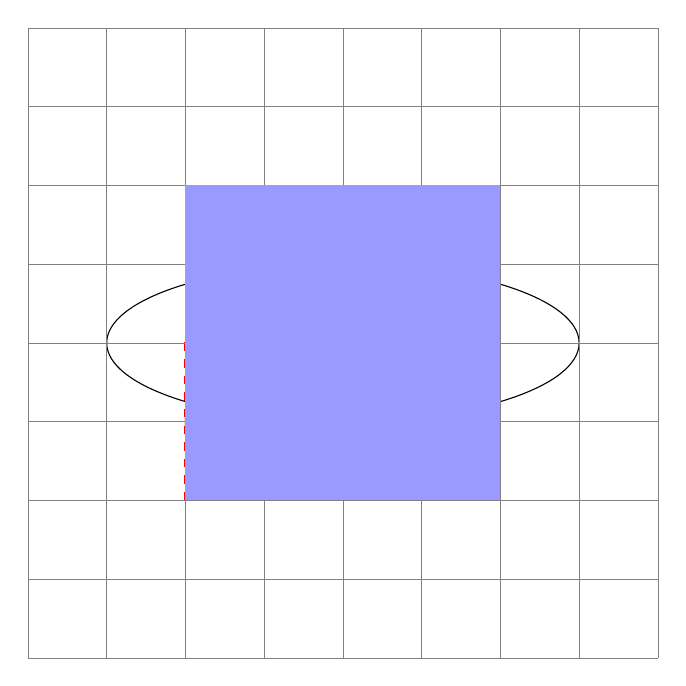
\begin{tikzpicture}
    \draw[red, thick, dashed] (0,0) rectangle (2,2);
    \pause % 
    \draw (1,1) circle [radius=1cm];
    \pause
    \draw (2,2) ellipse (3cm and 1cm);
    \pause
    \draw[step=1cm, gray,very thin] (-2,-2) grid (6,6);
    \pause
    \fill[blue!40!white] (0,0) rectangle (4,4);
    
  \end{tikzpicture}
  \end{center}
\end{frame}

\end{document}